\documentclass[french,a4paper,10pt,twocolumn]{article}
\usepackage{graphicx} % Required for inserting images
\usepackage[style=authoryear, backend=biber]{biblatex}
\usepackage[left=1cm,right=1cm,top=1cm,bottom=2cm]{geometry}
\usepackage[style=authoryear, backend=biber]{biblatex}
\usepackage{hyperref}
\usepackage{csquotes}
\usepackage{animate}
\usepackage[T1]{fontenc}
\usepackage{amsmath}
\usepackage[french]{babel}
\usepackage{array}
\usepackage{listings}
\usepackage{booktabs}
\usepackage[table,xcdraw]{xcolor}
\usepackage{float}
\usepackage{subcaption} % Pour les sous-figures

% Configuration du style pour Python
\lstdefinestyle{python}{
    language=Python,
    basicstyle=\ttfamily,
    numbers=left,
    numberstyle=\tiny,
    frame=single,
}

% Configuration du style pour Bash
\lstdefinestyle{bash}{
    language=Bash,
    basicstyle=\ttfamily,
    numbers=left,
    numberstyle=\tiny,
    frame=single,
}

\title{PRO3600: Mars Lander}
\author{Augustin Bresset | Zacharie March}
\date{January 2024}
\addbibresource{references.bib} %Imports bibliography file

\begin{document}
\onecolumn
\maketitle

\begin{figure}[H]
    \centering
    
\includegraphics[scale=0.2]{images/logo-tsp-fond-blanc.png}
    \caption{Logo TSP}\label{fig:logo}
\end{figure}

\tableofcontents
\pagebreak
\section{Introduction}

\subsection{Présentation du problème: Mars Lander}

Mars Lander est un problème d'optimisation proposé sur la plateforme \cite[]{codingame_mars_lander}.
Ce jeu consiste en le contrôle du moteur d'un vaisseau spatial (puissance des moteurs, angles de rotation) 
afin de le faire atterrir en toute sécurité et en douceur sur une surface plane de la planète Mars. 
L'idée est donc de trouver une trajectoire fonctionnelle. Ce problème est un classique de l'optimisation et de l'intelligence artificielle,
on lui retrouve des solutions basées sur de nombreuses approches très différentes.

\subsubsection{Environnement}

La surface de Mars est représenté localement par une suite continue de segments.
Parmis ces segments, un seul est rigouresement vertical, celui-ci définit la zone d'atterissage que la navette doit viser.
Au moindre contact avec la surface, le vaisseau atterit et le jeu est terminé.


\begin{figure}[H]
    \centering
    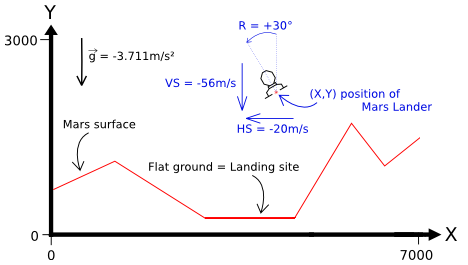
\includegraphics[scale=0.5]{images/marslander.png}
    \caption{Schéma du problème}\label{fig:marslander}
    \cite[]{codingame_mars_lander}
\end{figure}

\subsubsection{Espace des Etats}

Le vaisseau est représenté comme un propulseur à 
L'état du vaisseau est représenté par un vecteur de 7 valeurs:

\begin{figure}[H]
    \centering
    \begin{tabular}{|c|c|c|}
        \hline
        \textbf{Paramètre} & \textbf{Description} & \textbf{Bornes} \\
        \hline
        $x$       & position horizontale & $[0, 7000]$ \\
        \hline
        $y$       & position verticale   & $[0, 3000]$ \\
        \hline
        $hSpeed$  & vitesse horizontale  & - \\
        \hline
        $vSpeed$  & vitesse verticale    & - \\
        \hline
        $fuel$    & quantité de carburant restante & $[0, \infty[$ \\
        \hline
        $rotate$  & angle de rotation    & $[-90, 90]$ \\
        \hline
        $power$   & puissance des moteurs & $[0, 4]$ \\
        \hline
    \end{tabular}
\end{figure}


\subsubsection{Espace des Actions}

Toutes les secondes, en fonction des paramètres d’entrée (position, vitesse, fuel, etc.), 
le programme doit fournir le nouvel angle de rotation souhaité ainsi que la nouvelle puissance des fusées de Mars Lander.
Mais les commandes de puissance des fusées et de l’angle de rotation sont bornés.
La rotation est limitée à $[-15, 15]$ degrés et la variation de puissance des moteurs est limitée à $\{-1, 0, +1\}$.

\begin{figure}[H]
    \centering
    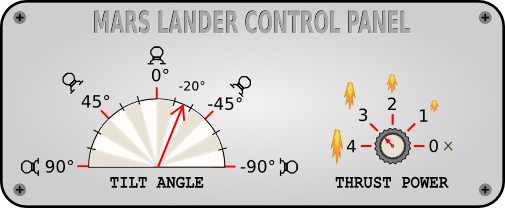
\includegraphics[scale=0.5]{images/ControlPanel.png}
    \caption{Figure du tableau de commande}\label{fig:control_panel}
    \cite[]{codingame_mars_lander}
\end{figure}

\subsubsection{Conditions d'atterrissage}

Afin de considérer qu'un attérissage est réussi, il faut respecter les conditions suivantes:
\begin{itemize}
    \item atterrir dans la \textbf{zone d'atterissage}
    \item atterrir en \textbf{position verticale} (angle d'inclinaison = 0°)
    \item la \textbf{vitesse verticale} doit être limitée ($\le 40m.s^{-1}$ en valeur absolue)
    \item la \textbf{vitesse horizontale} doit être limitée ($\le 20m.s^{-1}$ en valeur absolue)
\end{itemize}

\subsection{Algorithme Génétique}

Afin de résoudre ce problème, nous avons choisi d'utiliser une approche heuristique, les algorithmes génétiques.

Les algorithmes génétiques sont des algorithmes d'optimisation stochastique inspirés de la théorie de l'évolution naturelle.
Ils sont basés sur le principe de \textbf{sélection naturelle}.\\
Dans un premier temps on génère une \textbf{population} de solution aléatoire, on simule ensuite ces solutions et on calcule un \textbf{score} pour chacune d'entre elles.
On fait ensuite évoluer cette population à travers des phénomènes semblables à la sélection naturelle tel que la \textbf{sélection}, la \textbf{reproduction} et la \textbf{mutation}.
On répète ce processus jusqu'à ce qu'une solution satisfaisante soit trouvée.
Dans notre problème, une solution est définie par une trajectoire, c'est à dire une suite de commande à effectuer par le vaisseau.\\

\begin{figure}[H]
    \centering
    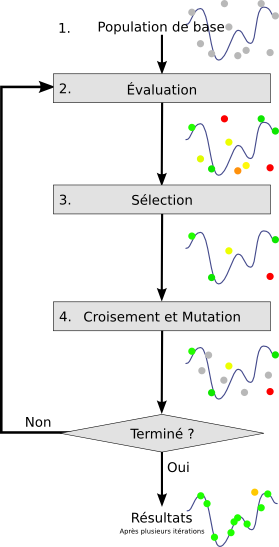
\includegraphics[scale=0.5]{images/schema_simple_algorithme_genetique.png}
    \caption{\cite[Schéma du fonctionnement de l'algorithme génétique]{schema_genetic_algorithm_image}}\label{fig:genetic_algorithm}
\end{figure}

\subsection{Objectif}

L'objectif de ce projet est de développer un support sur lequel il sera possible de simuler, manipuler et visualiser les trajctoires de notre navette sur 
différentes cartes.
De plus on souhaite pouvoir appliquer nos propres solutions informatiques à ce problème et notamment l'algorithme génétique et lui dédier une visualisation adaptée
afin de bien étudier le problème et l'influence des hyperparamètres de la solution.
Pour cela on à définit plusieurs points afin de mener à bien notre projet: 
\begin{itemize}
    \item Création d'une \textbf{interface graphique} sur pygame
    \item Mise en place d'une \textbf{interface client} permettant de piloter la navette
    \item Calcul de \textbf{solution} notamment à l'aide d'algorithme génétique    
    \item Regrouper les fonctionnalités à l'aide d'un \textbf{menue}
\end{itemize}

\subsubsection{Cahier des charges}

Développer une applicattion avec interface graphique. Les fonctionnalités attendues sur l'application sont les suivantes:
\begin{itemize}
    \item Interface graphique avec menue
    \item Choix de la solution à utiliser
    \item Choix de la carte à utiliser
    \item Visualisation adapté à la solution utilisée
    \item Exécution de la simulation
\end{itemize}

Notre application sera de sorte à ce que l'on puisse facilement ajouter des solutions, des cartes et autres tel que des obstacles dynamiques.
Pour cela l'architecture devra s'inscrire dans une logique agile et modulaire.
On compte tester notre environnement à l'aide de tests unitaires et fonctionnels afin de vérifier la bonne dynimique de notre environnement en le comparant
à des environments déjà existants tel que celui issu de \cite[CodinGame]{codingame_mars_lander}.

L'objectif final étant d'avoir une plateforme sur laquelle il est facile de développer et tester des solutions à ce problème.
C'est pourquoi le langage \textbf{Python} est proposé pour ce projet, il permet de développer facilement des solutions et de les tester rapidement. 

\subsection{Organisation du projet}

\subsubsection{Répartition des tâches}

En claire la répartition des tâches est la suivante:
\begin{itemize}
    \item \textbf{Augustin Bresset}\\
        Développement de l'environnement et des solutions 
    \item \textbf{Zacharie March}\\
        Développement de l'interface graphique et de l'interface client
\end{itemize}
Dans les deux cas, un apprentissage de la librairie pygame est nécessaire. Que ce soit pour la création de la solution "manuelle" (contrôle par l'utilisateur)
ou pour la création de l'interface graphique.

\begin{table}[h!]
    \centering
    \caption{Répartition des heures dans la création d'un projet informatique}
    \begin{tabular}{|>{\raggedright}m{5cm}|c|c|}
        \hline
        \textbf{Phase} & \textbf{Augustin Bresset (heures)} & \textbf{Zacharie March (heures)} \\
        \hline
        Organisation & 2 & 2 \\
        \hline
        Apprentissage & 4 & 12 \\
        \hline
        Développement & 22 & 20 \\
        \hline
        Débogage et tests & 14 & 11 \\
        \hline
        Rédaction des livrables et autres documents & 8 & 6 \\
        \hline
        Total & 50 & 51 \\
        \hline
    \end{tabular}
    \label{tab:repartition_heures}
\end{table}

On a passé beaucoup de temps a coder ensemble car on a un niveau très hétérogène et le pair programming nous a permis de progresser plus rapidement sans en laisser 
un derrière. D'où la raison des commits qui sont toujours fait pas l'un des membres du groupe, cela n'est pas représentatif du travail fourni par chacun.

\subsubsection{Outils de travail}

Afin de communiquer, nous nous reposons pour la communication active sur plusieurs outils, étant deux,
nous n'étions pas restreint par le besoin de créer un groupe sur un outil de communication particulier tel que \textbf{Discord} ou \textbf{Slack}.
Pour la commun passive nous avons créée une organization sur Github dans laquelle on peut trouver deux repertoire:
\begin{itemize}
    \item \textbf{backend}: Contient le code source du projet
    \item \textbf{meta}: Contient la documentation du projet (et ce livrable)
\end{itemize}

Nous souhaitons aussi travailler en \textbf{pair programming} le plus possible afin de faciliter la communication et la compréhension du code.


\section{Développement}

\subsection{Architecture du projet}

Afin de mener notre projet à bien, nous avons décidé de découper le code en plusieurs modules.
\begin{figure}[H]
    \centering
    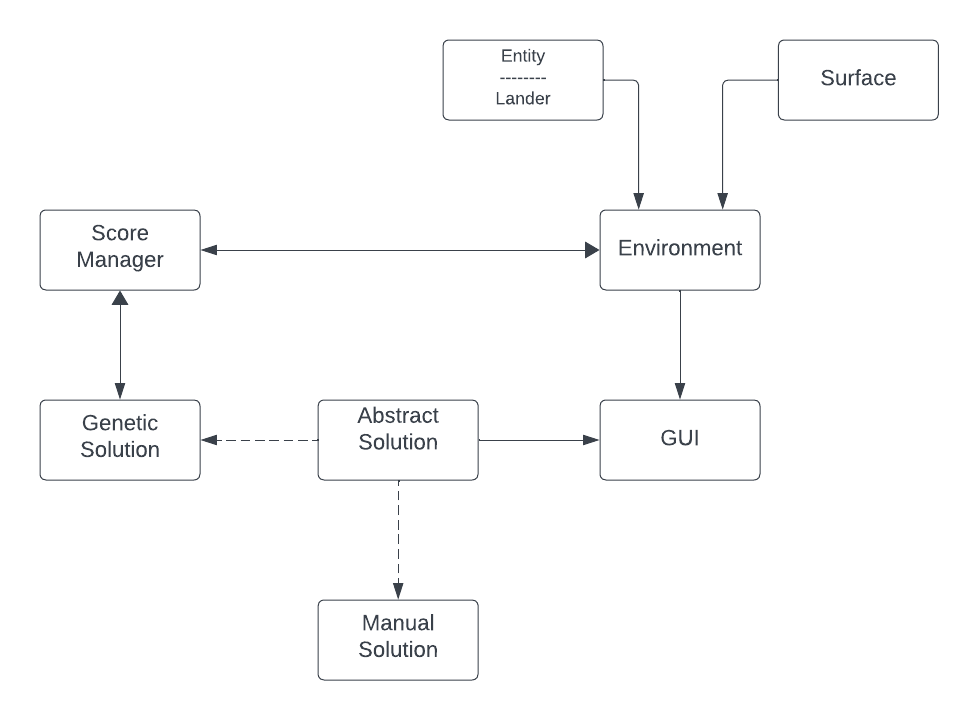
\includegraphics[scale=0.5]{images/class_diagram.png}
    \caption{Diagramme d'instance}\label{fig:architecture}
    \captionsetup{justification=centering, font=small}
    \caption*{Représente les interactions entre les différents objets}
\end{figure}

La figure \ref{fig:architecture}, nous présente les interactions entre les différents modules du projet.
Les flèches représentent les dépendances entre les modules. Par exemple \textit{Environment} dépend de \textit{Lander} et \textit{Surface}.
Chaque module et ces sous-modules ont une responsabilité bien définie.
Cette architecture a été pensé de manière agile, l'idée est donc de séparer les responsabilités au bon moment. 
Tout d'abord, la séparation de l'\textbf{environnement} et de la \textbf{Surface} permet un ajout de surface plus complexe avec des formes plus variées.
De même pour \textbf{Entity} qui est ici utilisé seulement pour le \textbf{Lander} mais qui pourrait être utilisé pour d'autres entités tel que des obstacles dynamiques.
Ensuite on a fait de même pour les \textbf{Solutions}, on a inscrit les commandes manuelles comme un type de solution à ce \textit{problème} afin de 
l'utiliser de la même manière que des solutions informatiques tel que l'algorithme génétique implémenté dans \textbf{GeneticSolution}.
Enfin la séparation de l'interface graphique \textbf{GUI} et du \textbf{ScoreManager} avec l'\textbf{Environment} permet une plus grande maniabilité dans le
développement de solutions qui fonctionne par apprentissage. En effet, on peut simuler des trajectoires sans avoir besoin de l'interface graphique et donc 
sans être limité par les performances de celle-ci et les FPS.

\subsubsection{Environnement}

Comme vu sur le diagramme, l'environnement instancie un \textbf{Lander} et une \textbf{Surface} et permet de simuler la trajectoire du vaisseau.
Il calcule les états dynamiques du système à chaque instant et permet de savoir si le vaisseau est en collision avec la surface et si il est sur la zone d'atterissage. 
Il implémente les méthodes suivantes:

\begin{itemize}
    \item \textbf{reset}: remet à zéro les paramètres dynamiques du vaisseau
        \item \textbf{exit\_zone}: vérifie si le vaisseau est sorti de la carte
        \item \textbf{landing\_on\_site}: vérifie si le vaisseau est sur la zone d'atterissage
        \item \textbf{landing\_angle}: vérifie si l'angle du vaisseau est correct
        \item \textbf{landing\_vertical\_speed}: vérifie si la vitesse verticale du vaisseau est correcte
        \item \textbf{landing\_horizontal\_speed}: vérifie si la vitesse horizontale du vaisseau est correcte
        \item \textbf{successful\_landing}: vérifie si l'atterissage est réussi
        \item \textbf{next\_dynamics\_parameters}: calcule les paramètres dynamiques du vaisseau à l'instant suivant
        \item \textbf{step}: calcule les états du vaisseau à l'instant suivant et met à jour les paramètres dynamiques
\end{itemize}


Le \textbf{Lander} est une classe de données qui permet de représenter l'état du vaisseau à un instant donné
mais ce n'est pas le cas de \textbf{Surface} qui implémente \textbf{tey\_collide} qui détermine si une trajectoire est en collision avec la surface 
et retourne le segment de surface dans ce cas là.

Enfin on a définit trois cartes différentes stockées dans des fichiers json, par exemple la carte \texttt{level\_one.json} est définie comme suit:

\begin{lstlisting}
{   
    "name": "Level one",
    "points" : [[0, 100], [1000, 500], [1500, 100], [3000, 100], [5000, 1500], [6999, 1000]],
    "lander_state" : {
        "x" : 2500,
        "y" : 2500,
        "h_speed" : 0, 
        "v_speed" : 0,
        "fuel" : 1000,
        "rotate" : 0,
        "power" : 0
    }
}
\end{lstlisting}

Ainsi pour définir une carte il suffit de définir dans un fichier json, son \textbf{name}, les \textbf{points} qui définissent la surface et l'état initial du vaisseau.

\subsubsection{Gui}

L'interface graphique dépend de la solution adoptée, c'est pourquoi on a une class abstraite \textbf{GuiAbstract} qui permet de définir les méthodes communes à toutes les interfaces graphiques.
Les méthodes implémenté sont les suivantes:
\begin{itemize}
    \item \textbf{screen\_reset}: Réinitialise l'écran de l'interface graphique.
    \item \textbf{render\_reset}: Réinitialise effaçant tous les éléments affichés.
    \item \textbf{reset}: Réinitialise les paramètres dynamiques du vaisseau et de la surface.
    \item \textbf{display\_text}: Affiche du texte à l'écran de l'interface graphique.
    \item \textbf{draw\_surface}: Dessine la surface sur l'écran de l'interface graphique.
\end{itemize}
Méthodes abstraites:

\begin{itemize}
    \item \textbf{write\_parameters}: Écrit les paramètres de la solution dans un fichier.
    \item \textbf{step}: Effectue une étape de simulation de la trajectoire du vaisseau.
    \item \textbf{pygame\_step}: Effectue une étape de simulation de la trajectoire du vaisseau spécifiquement pour l'interface graphique pygame.
    \item \textbf{run}: Lance l'interface graphique et démarre la simulation.
\end{itemize}

Cette classe abstraite a permet l'implémtation d'une classe pour l'interface graphique \textbf{Gui} pour le pilotage manuel du vaisseau et 
une autre classe \textbf{GuiTrajectory} qui permet de visualiser plusieurs trajectoires simultanément, fonctionnalité utile pour visualiser par
population d'individus dans le cas de l'algorithme génétique.

\subsubsection{Solution}    

Une solution est définie par une classe abstraite \textbf{AbstractSolution} qui permet de définir les méthodes communes à toutes les solutions.
Elle demande l'implémentation des méthodes suivantes:
\begin{itemize}
    \item \textbf{get\_parameters}: retourne les paramètres de la solution
    \item \textbf{set\_parameters}: définit les paramètres de la solution
    \item \textbf{use} : envoi une instance d'action en fonction de l'envirronement
\end{itemize}

On a implémenté deux types de solutions:
\begin{itemize}
    \item \textbf{ManualSolution}: Solution manuelle permettant de piloter le vaisseau à l'aide du clavier
    \item \textbf{GeneticSolution}: Solution génétique permettant de piloter le vaisseau à l'aide d'un algorithme génétique
\end{itemize}

La solution manuelle est implémenté sans méthode supplémentaire, mais la solution génétique a besoin de plusieurs méthodes supplémentaires pour fonctionner.
Elle emploi notamment l'objet \textbf{Population} qui implémente toutes les méthodes liés à l'évolution: \textbf{selection}, \textbf{mutation}, ...
ainsi que des méthodes supplémentaires tel que la création d'une population aléatoire et une fonction de roulette cumulative.
Cette population créer un tableau de genome qui repondent à la classe abstraite \textbf{AbstractChromosome} qui permet de définir les méthodes communes à tous les chromosomes.
Une classe \textbf{ActionChromosome} a été implémenté pour ce problème, elle permet de définir les actions à effectuer par le vaisseau à un instant donné.
L'idée derrière l'emploi de classe abstraite est l'application d'algorithme génétique à d'autres paramètres du problème.

\subsubsection{Score}

Le module \textbf{ScoreManager} permet de calculer le score d'une trajectoire. Cette classe n'a aucun intérêt pour le mode manuel du vaisseau,
mais permet à l'aide d'un algorithme génétique de trouver la meilleure trajectoire possible.
Il implémente les méthodes suivantes:

\begin{itemize}
    \item \textbf{landing\_distance}: calule la distance au sol entre la zone de collision et la zone d'atterissage
    \item \textbf{scoring\_distance\_off\_site}: détermine un score en fonction de la distance au sol
    \item \textbf{scoring\_distance\_on\_site}: donne le score si le vaisseau est sur la zone d'atterissage
    \item \textbf{scoring\_speed\_on\_site}: détermine le score en fonction de la vitesse du vaisseau lors de l'atterissage dans le cas où le vaisseau est sur la zone d'atterissage
    \item \textbf{scoring\_speed\_off\_site}: détermine le score en fonction de la vitesse du vaisseau lors de l'atterissage dans le cas où le vaisseau n'est pas sur la zone d'atterissage
    \item \textbf{scoring\_angle}: détermine le score en fonction de l'angle du vaisseau lors de l'atterissage    
\end{itemize}

\subsubsection{Utils}

Le module \textbf{Utils} contient des fonctions utilitaires et des constantes utilisées dans les autres modules et notamment les classes
\textbf{Point} et \textbf{Segment}.

\textbf{Point}\\
La classe Point permet de représenter un point dans un espace à deux dimensions. Il lui ait associé des fonctions permettant de calculer la distance et de gérer
les égalités entre deux points. 
On a considérer ici que deux points étaient égaux si leurs coordonnées étaient assez proches.

\textbf{Segment}\\
La classe Segment permet de représenter un segment dans un espace à deux dimensions.
Sa méthode la plus utile est la méthode \textbf{collision} qui à l'aide d´une fonction \cite[\textbf{CCW}]{ccw_intersect_detection} qui permet de savoir si deux segments se croisent.

En considérant un instant de trajectoire comme étant un segment, on peut vérifier si il ne rentre pas en collision avec la surface grâce à cette méthode.

Enfin d'autre scripts ont permis le débuggage tel que \textbf{display\_map} ou bien \textbf{load\_map} qui permet de charger la carte.
\subsection{Tests}

Afin de vérifier le bon fonctionnement de notre code, nous avons mis en place des tests.
Ces tests se divisent en trois catégorites qui composent ces parties.
On va voir dans un premier temps les \textbf{tests unitaires} qui permettent de tester les fonctions et méthodes importantes et de manières indépendantes
au reste du code.
Il enn suivra les \textbf{tests d'intégration} qui permettent de tester le bon fonctionnement des modules entre eux.
Et enfin les \textbf{tests fonctionnels} qui permettent de tester le bon fonctionnement de l'application dans son ensemble.

Nous utiliserons la librairie \textbf{unittest} pour l'écriture de nos tests.

\subsubsection{Tests unitaires}

\textbf{Environnement}
Afin de tester l'environnement, nous avons récuperer les réponses dynimiques de l'environnement présent sur \cite[CodinGame]{codingame_mars_lander} 
et nous avons comparer les états à chaque instant à ceux calculer par notre environnement.\\
De plus on a fait des tests pour vérifier que les collisions avec la surface étaient bien détectées. 
Et notamment que les collisions avec avec le site d'atterissage est bien détecté et que si le vaisseau 
sort de la carte, ce soit bien détecté par l'environnement.


\textbf{Score}
Les fonctions étant simplement des fonctions mathématiques dépendant d'un paramètre du problème, nous n'avons pas jugé nécessaire de faire des tests unitaires
excepté pour la fonction qui permet de calculer la distance entre la zone de collision et la zone d'atterissage.
En effet, ce n'est pas une simple distance euclidienne, mais plutot la distance en suivant la surface de l'environnement.
On a pu vérifier le bon fonctionnement de cette fonction à l'aide de cas caculé à la main.
Et les trois tests nous permettent de nous laisser penser que :
\begin{itemize}
    \item La distance est bien décroissante si l'on se dirige vers la zone d'atterissage
    \item La distance est bien calculée
\end{itemize}

\textbf{Algorithme Génétique}
Ces tests unitaires sont destinés à évaluer le fonctionnement de certaines fonctionnalités de l'algorithme génétique mise en œuvre.

On test tout d'abord la génération d'une population. Il crée une population de 10 individus, chacun ayant 100 gènes du type "ActionChromosome". 
Les assertions comparent la longueur de la population, la longueur des gènes du premier individu, 
et s'assurent que la longueur des gènes est la même pour tous les individus, tout en vérifiant qu'il y a des différences entre les gènes des deux premiers individus.
    
Puis on test la \textbf{cumulative wheel}, ce test évalue la fonction qui génère une roue cumulative pour la sélection d'individus. 
Une population de 10 individus est créée avec des scores aléatoires. 
La population est triée en fonction des scores, puis la roue cumulative est générée. 
Les assertions vérifient que la longueur de la roue cumulative est correcte, 
et que chaque élément de la roue est une paire d'individus de type "ActionChromosome", avec des identifiants différents.

Enfin on vérifie \textbf{la sélection} du/des meilleur individu dans une population.Ce test évalue la fonction de sélection du meilleur individu dans une population. 
Une population de 10 individus est créée, chaque individu ayant un score égal à son index. La population est triée en fonction des scores,
et la meilleure solution est sélectionnée. Les assertions comparent le score de la meilleure solution avec l'index attendu, soit 9 dans ce cas.
En résumé, ces tests garantissent le bon fonctionnement de différentes parties de la solution génétique, y compris la génération de populations, la création de roues cumulatives pour la sélection, et la sélection du meilleur individu dans une population.

\subsubsection{Tests d'intégration et fonctionnels}
Les tests d'intégration et fonctionnels on plutôt été fait de manière empirique, c'est à dire que l'on a testé le bon fonctionnement des modules entre eux à l'aide de l'interface graphique.
On a pu ainsi vérifier que les solutions fonctionnaient bien avec l'environnement et que l'interface graphique fonctionnait bien avec les solutions notamment grâce aux logs ajoutés dans le prompt.

\begin{figure}[H]
    \centering
    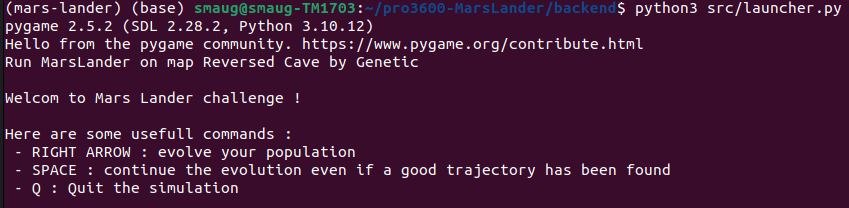
\includegraphics[scale=0.5]{images/log_prompt_menue.png}
    \caption{Exemple de logs}\label{fig:logs}
\end{figure}


\section{Résultats}

\subsection{Menue}
L'application est divisée en deux parties, le \textbf{menue} et la \textbf{partie}.

Dans le menue, on propose à l'utilisateur de choisir entre deux solutions : \textbf{Manual} et \textbf{Genetic} puis entre trois cartes prédéfinies : \textbf{level one}, \textbf{Reversed Cave} et \textbf{Flat Surface}.

\begin{figure}[H]
    \centering
    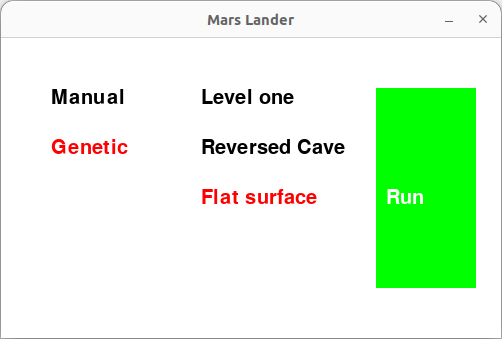
\includegraphics[scale=0.5]{images/menue.png}
    \caption{Menue}\label{fig:menue}
\end{figure}

Ce menue permet de choisir la solution et la carte à utiliser pour la simulation, il suffit enfin de cliquer sur le bouton \textbf{Run} pour lancer la partie.

\subsection{Partie}

Une partie est lorsque l'on choisit la solution manuelle, elle ce joue à l'aide des flèches du clavier.
Les commandes sont les suivantes:
\begin{itemize}
    \item \textbf{Flèche du haut}: Augmente la puissance des moteurs
    \item \textbf{Flèche du bas}: Diminue la puissance des moteurs
    \item \textbf{Flèche de gauche}: Tourne le vaisseau à gauche
    \item \textbf{Flèche de droite}: Tourne le vaisseau à droite
\end{itemize}

Une fois la partie lancé, on peut contrôler le vaisseau. Arriver au sol, le logiciel trace la trajectoire effectuer
et sa couleur indique le succès ou non de l'atterissage, vert pour un succès et bleu pour un échec.

\begin{figure}[H]
    \centering
    \begin{subfigure}[b]{0.3\textwidth}
        \centering
        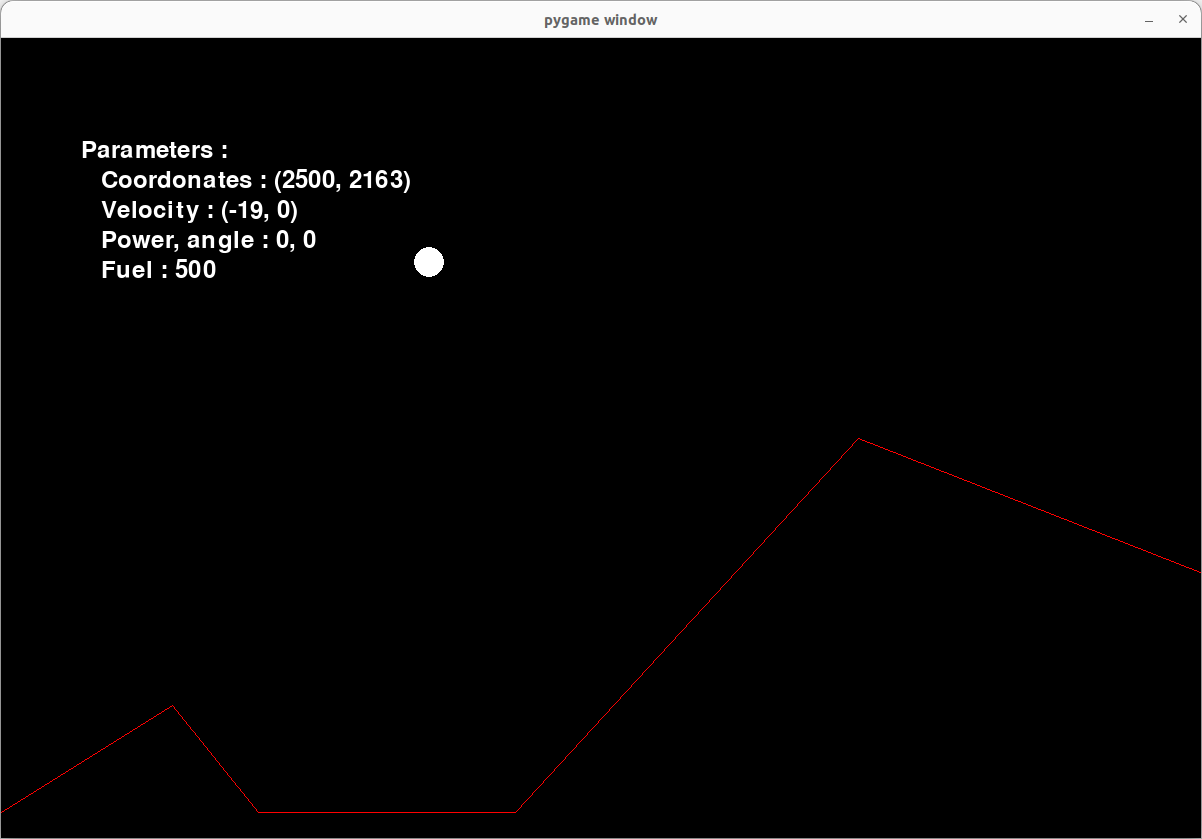
\includegraphics[width=\textwidth]{images/initial_lvl_one_manual.png}
        \caption{Début de partie en manuel}
    \end{subfigure}
    \hfill
    \begin{subfigure}[b]{0.3\textwidth}
        \centering
        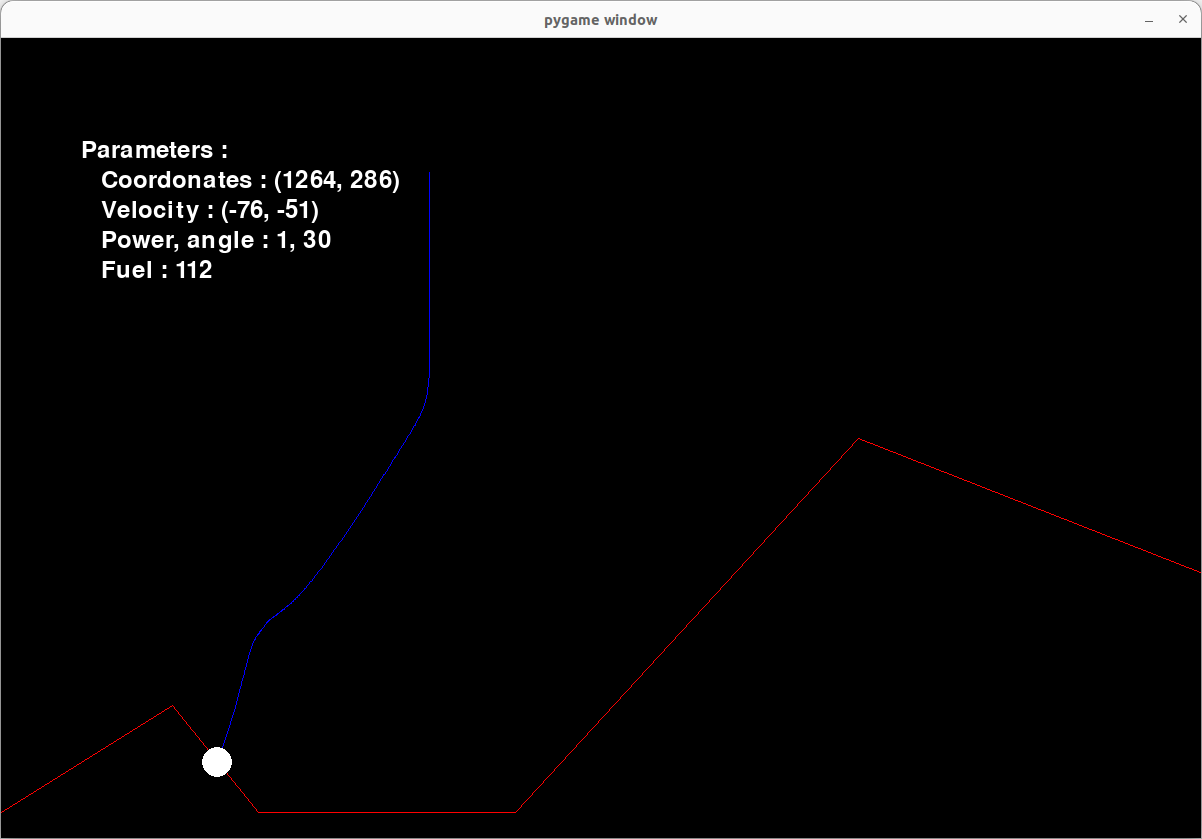
\includegraphics[width=\textwidth]{images/unsuccessfull_lvl_one_manual.png}
        \caption{Fin de partie avec crash}
    \end{subfigure}
    \hfill
    \begin{subfigure}[b]{0.3\textwidth}
        \centering
        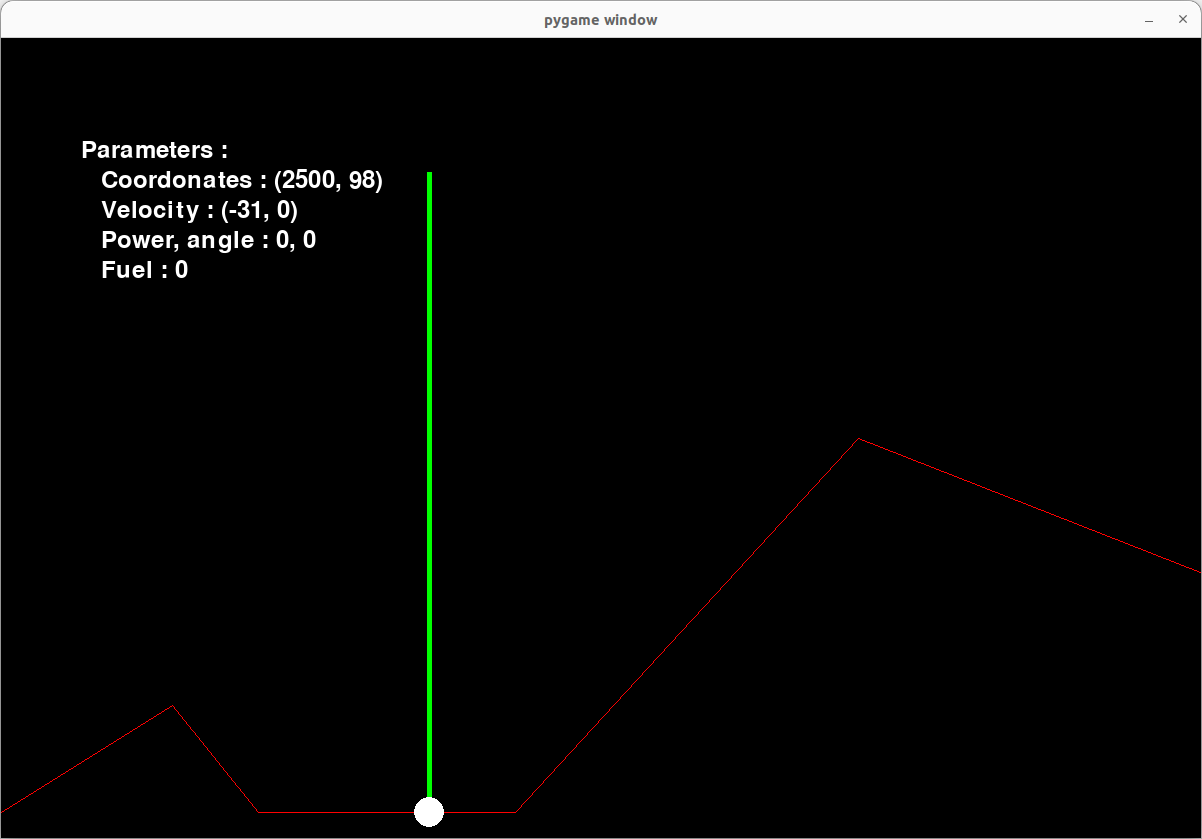
\includegraphics[width=\textwidth]{images/successful_lvl_one_manual.png}
        \caption{Fin de partie avec succès}
    \end{subfigure}
\end{figure}

Le vaisseau est représenté par un cercle blanc et la surface par des segments rouges.

\subsection{Simulation}

Pour représenter les résultats de l'algorithme génétique, on affiche les trajectoires population par population.
On peut ainsi voir l'évolution des trajectoires au fur et à mesure des générations.

\begin{figure}[H]
    \centering
    \begin{subfigure}[b]{0.45\textwidth}
        \centering
        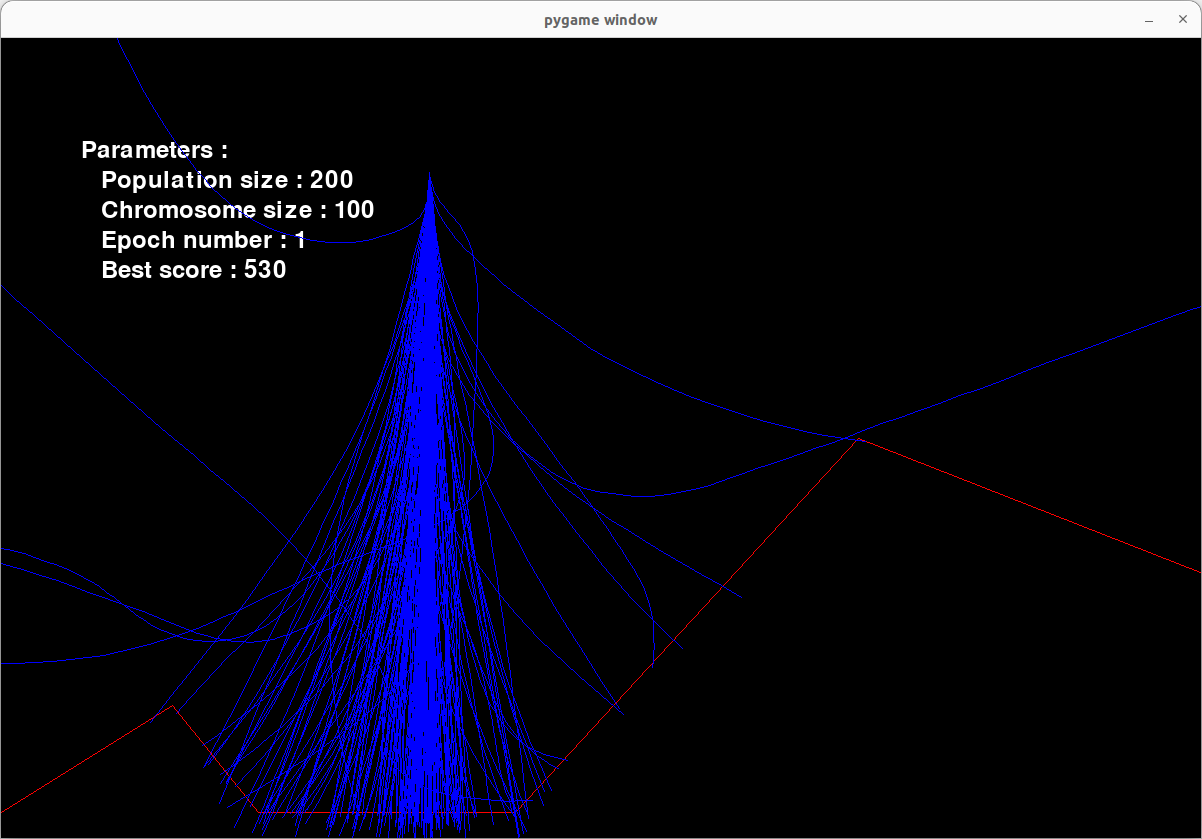
\includegraphics[width=\textwidth]{images/lvl_one_ga.png}
        \caption{Début de partie en génétique}
    \end{subfigure}
    \hfill
    \begin{subfigure}[b]{0.45\textwidth}
        \centering
        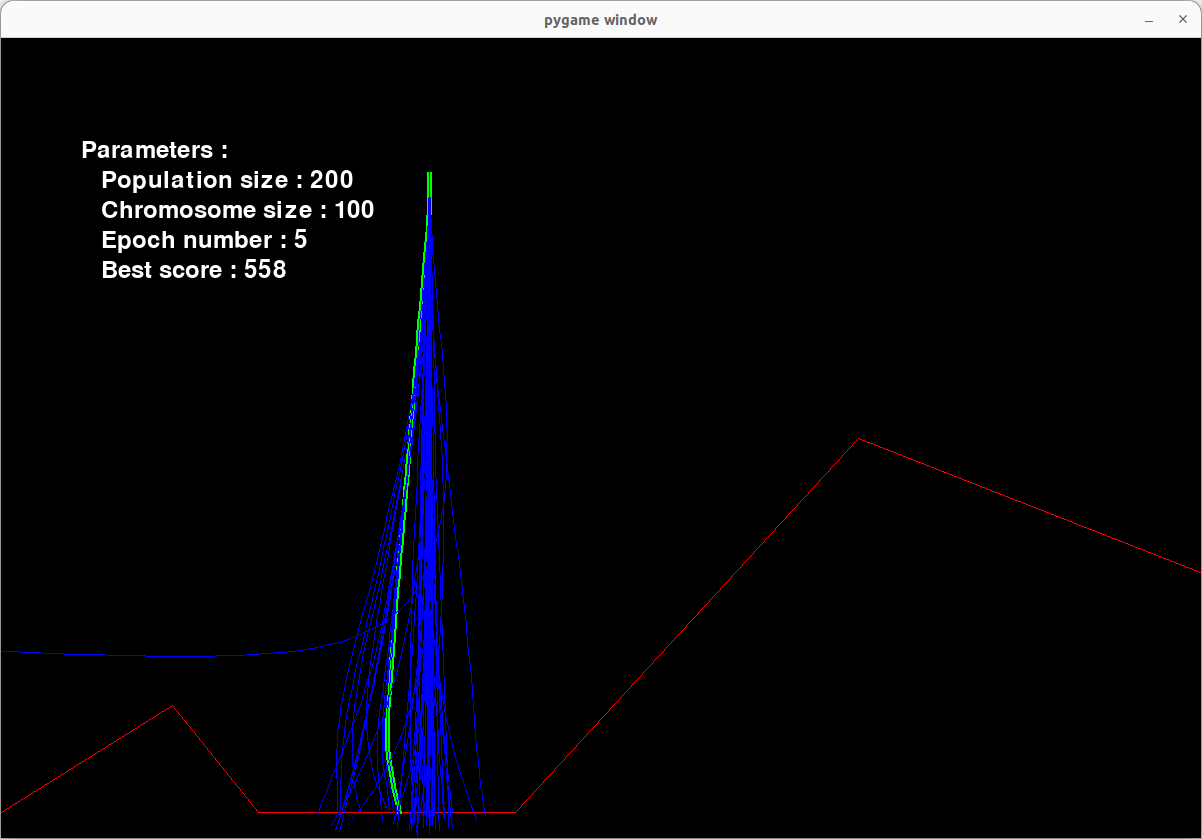
\includegraphics[width=\textwidth]{images/successful_lvl_one_ga.png}
        \caption{Fin de partie en génétique}
    \end{subfigure}
\end{figure}

On a aussi une carte plus compliquée, la \textbf{Reversed Cave} qui permet de tester la robustesse de notre algorithme génétique.

\begin{figure}[H]
    \centering
    \begin{subfigure}[b]{0.45\textwidth}
        \centering
        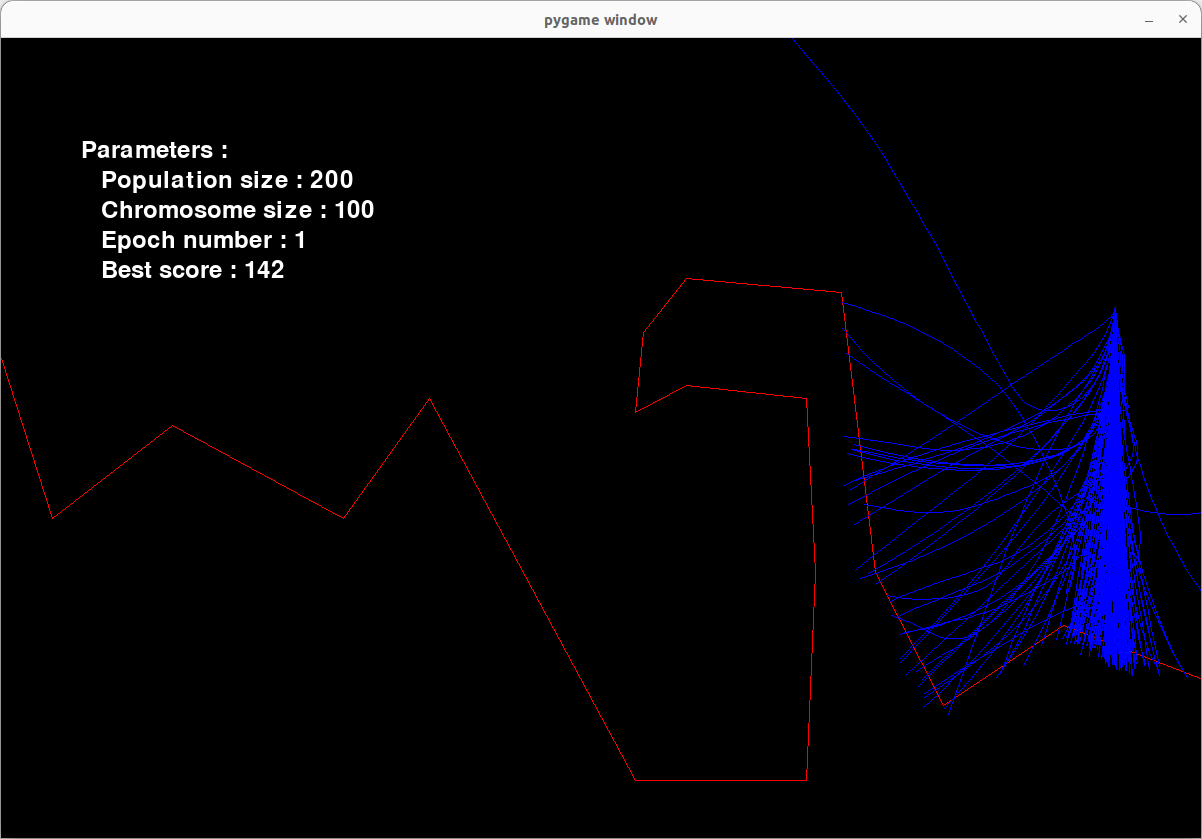
\includegraphics[width=\textwidth]{images/first_epoch_rc_ga.png}
        \caption{Début de partie en génétique}
    \end{subfigure}
    \hfill
    \begin{subfigure}[b]{0.45\textwidth}
        \centering
        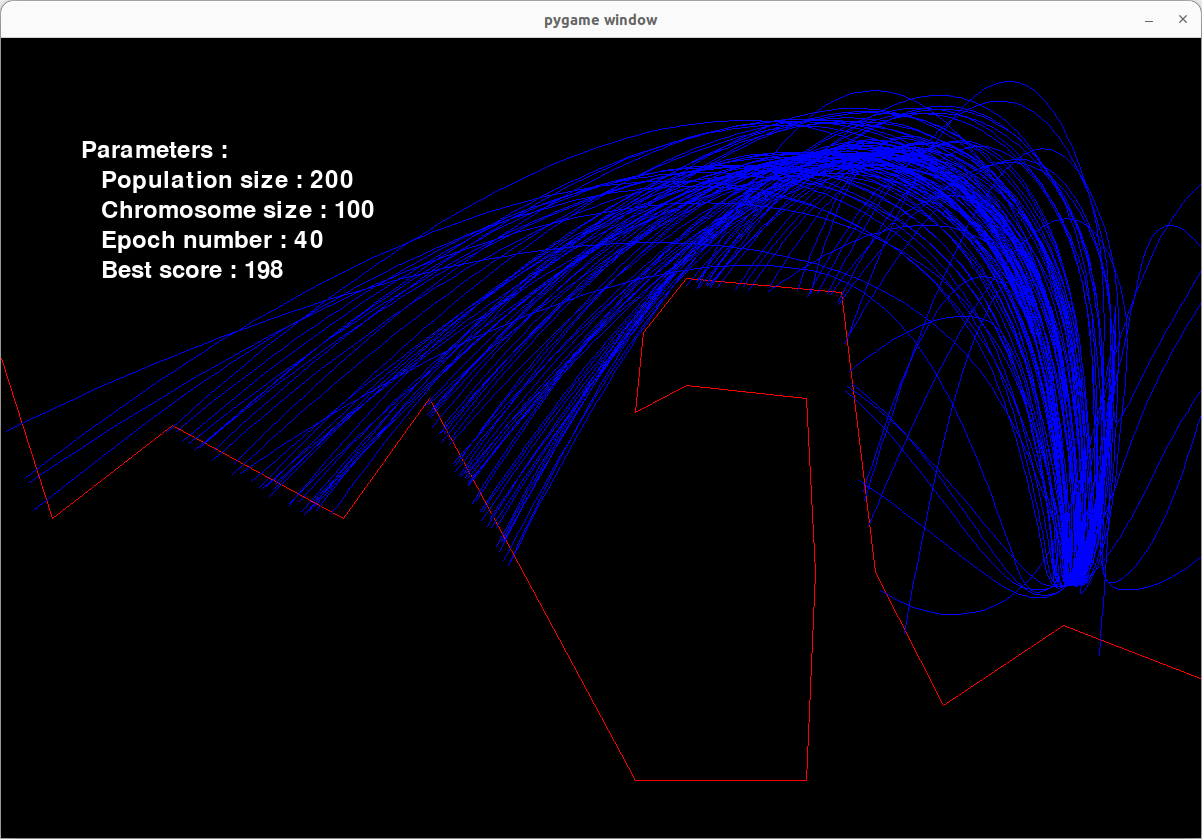
\includegraphics[width=\textwidth]{images/40_epoch_rc_ga.png}
        \caption{Simulation à l'époque 40}
    \end{subfigure}
    \hfill
    \begin{subfigure}[b]{0.45\textwidth}
        \centering
        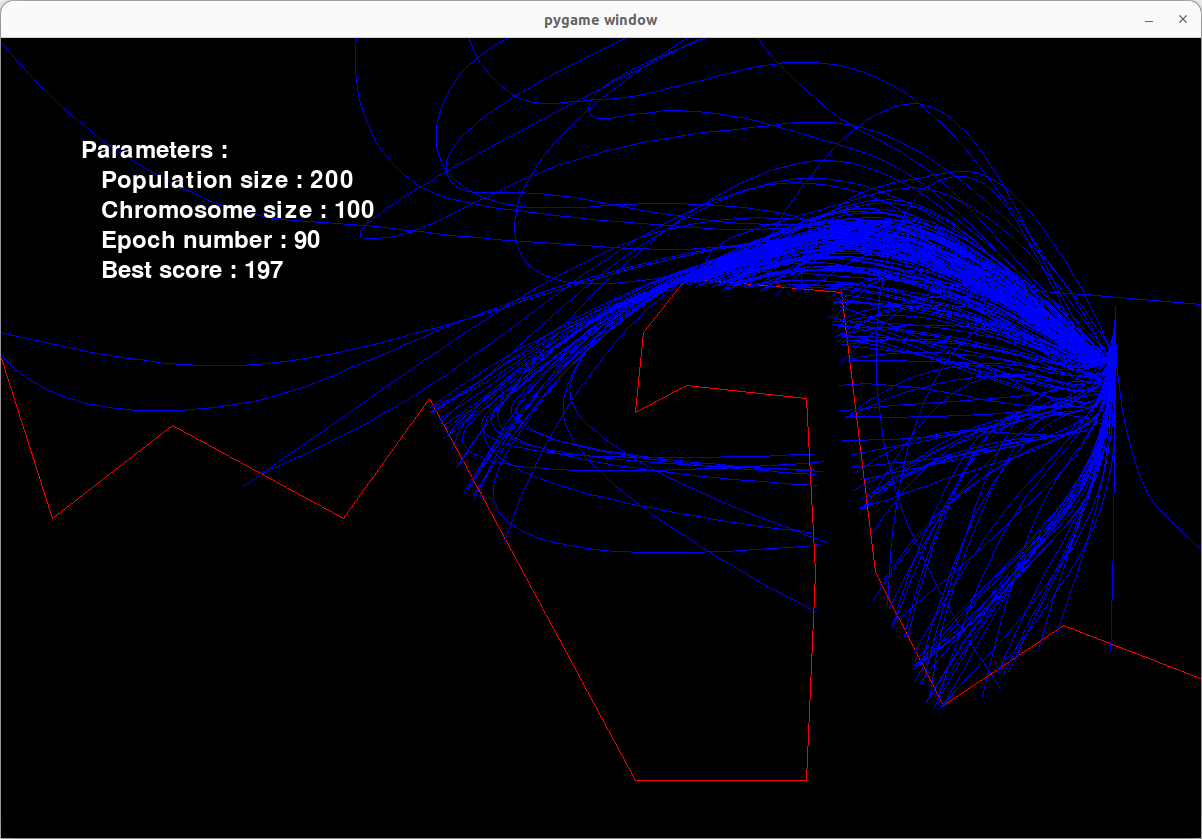
\includegraphics[width=\textwidth]{images/90_epoch_rc_ga.png}
        \caption{Simulation à l'époque 90}
    \end{subfigure}
    \hfill
    \begin{subfigure}[b]{0.45\textwidth}
        \centering
        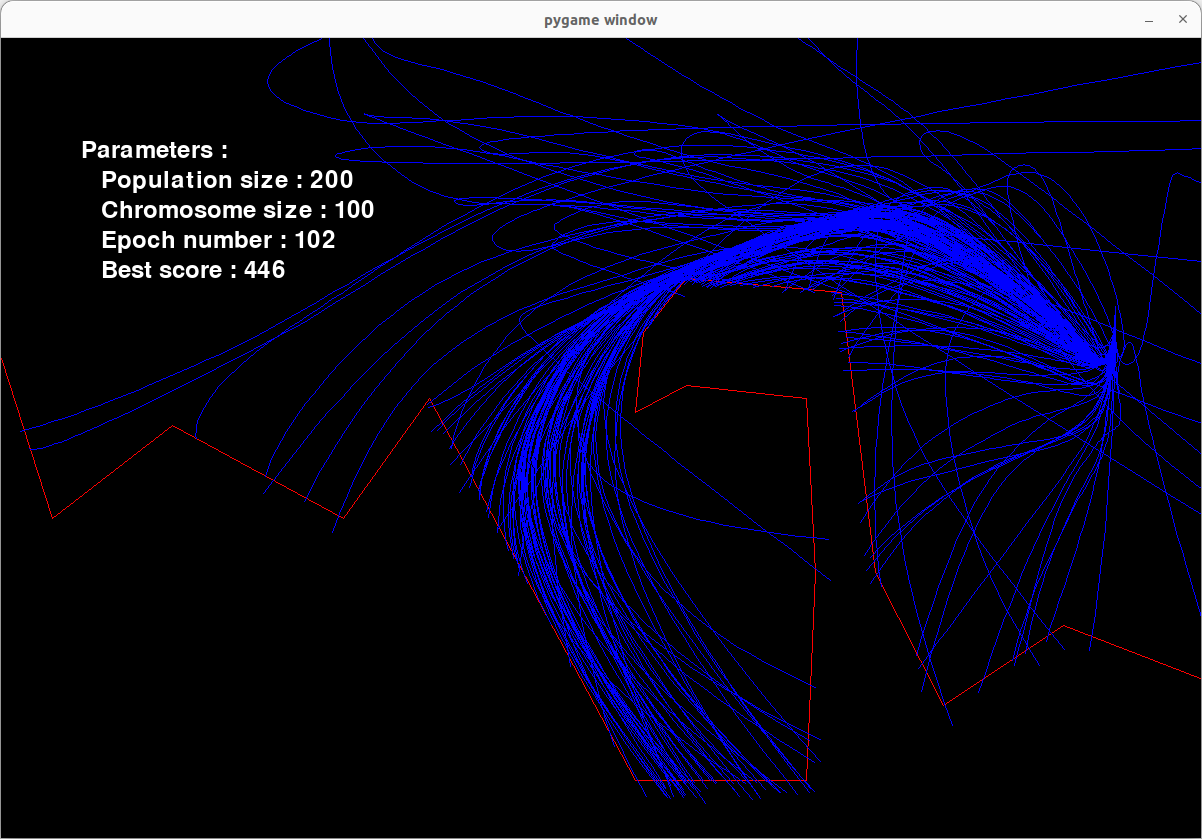
\includegraphics[width=\textwidth]{images/102_epoch_rc_ga.png}
        \caption{Simulation à l'époque 102}
    \end{subfigure}

\end{figure}

\subsection{Manuel utilisateur}

Afin de lancer le programme, il faut tout d'abord installer les dépendances du projet présentes dans le fichier \textbf{requirements.txt}.
Pour cela on peut utiliser la commande suivante:
\begin{lstlisting}[style=bash]
    pip install -r requirements.txt
\end{lstlisting}


Une fois les dépendances installées, on peut lancer le programme à l'aide de la commande suivante:
\begin{lstlisting}[style=bash]
    python src/launcher.py
\end{lstlisting}

\subsection{Critique et conclusion}
\subsubsection{Problèmes rencontrés}

Tout au long du projet, on a essayé de garder une architecture de code permettant une meilleure répartition des processus
tout en gardant une cohérence dans le code. 
Comme dit plus tôt, on a essayer de garder une structure agile, cela nous a prit du temps d'y réfléchir et de restructurer le code sans cesse.

Nous voulions diviser les repertoires github entre le frontend et le backend, mais nous avons finalement pas rencontrés ce besoins étant donné
que l'on travaillait sur le même langage. 

N'ayant pas de deadline claire, on a pu prendre le temps de bien réfléchir à l'architecture du code et à la répartition des tâches mais 
ca nous a aussi conduit a prendre plus de temps que nécessaire pour certaines tâches.
Finalement, on s'est remis à faire des deadlines pour pouvoir avancer plus rapidement.

\subsubsection{et amélioration à envisager}

On est fière d'avoir sur créer une architecture répondant à nos attentes et on aurait aimé prendre plus de temps à développer d'autres solutions 
qu'elle soit sur les algorithmes génétiques ou sur d'autres types de solutions.

Dans l'interface graphique, on aurait aimé ajouté un menue supplémentaire permettant de modifier directement les paramètres du jeu sans passer par le code.
On aurait aussi aimé ajouter des obstacles dynamiques pour rendre le jeu plus intéressant.

Finalement d'un point de vue optimisation, notre jeu aurait pu être bien plus performant si on avait forcé l'utilisation de numpy et numba pour les calculs 
mais n'étant tous les deux pas du mêmes niveau en python, on a préféré ne pas le faire et surtout que le jeu est déjà assez rapide pour être jouable.

\printbibliography
\end{document}
